\documentclass{article}
\usepackage{styles}

%%%%%%%%%%%%%%%%%%%%%%%%%%%%%%%%%%%%%%%%%%%%%%%%%%%%%%%%%%%%%%%%%%%%
%%--------------------------GLOSSARY------------------------------%%
%%%%%%%%%%%%%%%%%%%%%%%%%%%%%%%%%%%%%%%%%%%%%%%%%%%%%%%%%%%%%%%%%%%%

\makenoidxglossaries
\newacronym{rfe}{RFE}{Recursive Feature Elimination}
\newacronym{cv}{CV}{Cross-Validation}
\newacronym{dt}{DT}{Decision Tree}
\newacronym{lasso}{LASSO}{Least Absolute Shrinkage and Selection Operator}
\newacronym{pca}{PCA}{Principle Component Analysis}
\newacronym{lda}{LDA}{Linear Discriminant Analysis}
\newacronym{knn}{k-NN}{k- Nearest Neighbors}
\newacronym{nb}{NB}{Naïve Bayes}
\newacronym{svd}{SVD}{Singular Value Decomposition}
\newacronym{ml}{ML}{Machine Learning}
\newacronym{ai}{AI}{Artificial Intelligence}
\newacronym{pcc}{PCC}{Pearson product-moment Correlation Coefficient}

\newglossaryentry{apriori}
{
    name={apriori},
    description={\textit{Apriori} information refers to any possible information about the dataset feature importances one has before running any learning algorithms. Common ways to obtain such information are human domain experts or the usage of synthetic datasets}
}

\newglossaryentry{ib1}
{
  name={IB1},
  description={Instance-based classification algorithm originally proposed by Aha et al. (1991) \citep{aha_instance-based_1991}},
  first={\glsentrytext{ib1}},
  plural={IB1},
  firstplural={\glsentrytext{ib1}}
}

\newglossaryentry{part}
{
  name={PART},
  description={Partial Decision Tree algorithm},
  first={\glsentrytext{part}},
  plural={PART},
  firstplural={\glsentrytext{part}}
}

\newglossaryentry{rba}
{
  name={RBA},
  description={Relief-Based Feature Selection Algorithms},
  first={\glsentrydesc{rba} (\glsentrytext{rba})},
  plural={RBAs},
  firstplural={\glsentrydesc{rba}s (\glsentryplural{rba})}
}

\newglossaryentry{svm}
{
  name={SVM},
  description={Support Vector Machine},
  first={\glsentrydesc{svm} (\glsentrytext{svm})},
  plural={SVMs},
  firstplural={\glsentrydesc{svm}s (\glsentryplural{svm})}
}


%%%%%%%%%%%%%%%%%%%%%%%%%%%%%%%%%%%%%%%%%%%%%%%%%%%%%%%%%%%%%%%%%%%%
%%-----------------------DOCUMENT BEGIN---------------------------%%
%%%%%%%%%%%%%%%%%%%%%%%%%%%%%%%%%%%%%%%%%%%%%%%%%%%%%%%%%%%%%%%%%%%%
\begin{document}

\begin{titlepage}
    \thispagestyle{empty}
    \title{
        
\includegraphics[width=19cm]{images/rug_fse_cs_logo.pdf} \\
        \vspace{3cm}
        \begingroup
        \setstretch{4}\fontsize{38}{10}\selectfont\fontdimen2\font=0.8ex
        \parbox{13.3cm}{\textBF{Evaluating the performance of supervised feature ranking algorithms on tabular feature datasets.}} %%Title
    \endgroup}
    \date{June 2021, Draft 1/2}
    \author{J.G.S. Overschie}
    \maketitle
    \vspace{-7.5cm}
    \hspace{4cm}\parbox[b][15cm][b]{8cm}{\textDF{\large\setstretch{1.5}
    MSc Thesis INMSTAG-08\\
    Student: J.G.S. Overschie\\ %NAME
    First supervisor: dr. G. Azzopardi\\
    Second assessor: A.M.J.A. Alsahaf}}
\end{titlepage}
\newpage
\newgeometry{top=1in,bottom=1in,right=1.25in,left=1.25in} %Needed because margins were changed for titlepage

\hrule
\begin{abstract}
\end{abstract}
\hrule

\tableofcontents

\newpage
\section{Introduction}\label{section:introduction}
% more data: many domains
In this day and age, more data is available than ever before in many domains \citep{sagiroglu_big_2013}. In the biomedical domain sensory devices such as MRI or PET scanners are getting ever more accurate - requiring more storage space to store higher resolution data; in the financial domain markets are operating at increasingly low time intervals - requiring storage and analysis of data at a higher time resolution than before and lastly; the internet is increasing in amount of traffic on a global scale and is producing immense amounts of data. Applications of Machine Learning are common in all these domains: training predictive models by learning from example data is able to give us interesting insights that can improve both economy and the quality of human lives. By the nature of models that learn from examples, performance is often better when a larger amount of examples is available. But it shall get clear that larger quantities of data presents itself not as solely beneficial; but rather- a mixed blessing.

% ML can benefit: but also harder.
The field of Machine Learning has seen vast increases in dataset sizes: both in terms of sample size and amount of dimensions. But although the availability of more data presents practitioners opportunities to create better performing models, more data will have to be processed - causing an increased computational burden in the learning process. Which increase is nonlinear: due to the curse of dimensionality, the computational burden can get large, quickly. Even though the field has for long relied on computer processing speed steadily increasing, obeying Moore's law, the rate of advancement will inevitably start declining - and in fact already has \citep{theis_end_2017}. Self-evidently, many technological advancements can still be realised, be it either in the silicon world or in a post-silicon world, in which perhaps forms of quantum computing might become predominant \citep{britt_high-performance_2017}. But what is certain, is that besides the technological opportunities the chip-making industry still has, there also exist strict physical limitations as to how fast computer processing can get. So, besides leveraging faster hardware, we are also going to have to make our software smarter. Instead of increasing just our computational power, methods for reducing the computational burden in the first place are desired. Thus, the need for preprocessing techniques and data reduction algorithms is instigated.

% Feature Selection
\textbf{Feature selection} is such a domain that focuses on reducing the overall learning processing burden \citep{guyon_introduction_2003}. By figuring out what dimensions are relevant to the learning task, which ones are redundant, and which ones are completely noise with respect to the learning task, a smaller dataset can be obtained by means of a preprocessing step. This is contrary to the domain of dimensionality reduction, in which data is projected onto a space of smaller dimensionality - but losing the exact representation of the data distribution. In Feature Selection, we aim to obtain a binary decision about which dimensions to keep, in the original data space. Aside from reducing dataset size by cutting off dimensions, in some cases the generalization ability of a learning model can even be improved: the learning model can better learn the data distribution by using less but more meaningful dimensions with less noise. This makes the benefit of learning on a subset of the available features two-fold: model fitting and prediction can be both faster and more accurate. To select relevant dataset features, a wide variety of strategies exist. One is to assign a scoring to each dimension and keep only the most relevant ones - such a ranking is called a feature ranking.

% Feature Ranking
\textbf{Feature ranking} is a broader domain in contrast to feature selection, in which the sole purpose is not to only reduce the dataset size, but to construct a hierarchical order on the importance of features given a specific learning task \citep{duch_comparison_2004}. Many techniques can be employed to create such feature rankings, of which some are substantially faster than others, but might yield sub-optimal results: the choice of a suitable feature ranking algorithm is not trivial in most scenarios. Once such a feature ranking has been constructed, it can be used for various applications. First, a feature selection can be made by cutting of features that rank below a certain feature importance score threshold; one naive such method would be to cut off any feature that ranks below the average feature importance score. Secondly, the feature ranking can also be used for better Machine Learning model interpretation; in which the feature importance scores help humans better understand the predictions and reasoning of the models - by knowing which features the model found important, it can better be understood how the model made the decision that it has. This second application is part of the bigger domain of Interpretable Artificial Intelligence, or more commonly \textit{Interpretable AI}, which has in recent times become ever more relevant \citep{ghosh_interpretable_2020} - aiming to explain models that were before considered `black box' models.

% Problem statement
\textbf{Evaluation} on the performance of feature ranking algorithms has been conducted in many different ways. Most authors used a `validation' estimator, which was trained on a chosen subset of the dataset to then see how the estimator performed given this feature subset. A ranker is desired, then, that ranks the most predictive features highest, preferably in a reasonable amount of time. In this way, we get a feature subset that is as small as possible, that gives us the highest possible predictive power. This evaluation technique, however, might not be systematic enough. Across papers, many different validation estimators are used, which make the results across papers subsequently incomparable to one another. Researchers might also benefit from more extensive and systematic evaluation by use of synthetic datasets. By manually controlling many aspects of the dataset, such as noise levels, the complexity of the data distribution to be learned and the amount of informative features, a comprehensive evaluation on the feature ranking algorithm behavior and characteristics can be made. In this way, by employing synthetic datasets, the exact informative features to be ranked as relevant can be known \textit{\gls{apriori}}, i.e. before conducting the feature ranking operation. Such new and possibly useful metrics can be employed to evaluate feature rankings independent of any validation estimator.

% In this paper
\textbf{In this paper}, a comprehensive comparative experiment on feature rankers is conducted using both real-world and synthetic datasets, employing new evaluation metrics on the synthetic datasets by knowing the relevant feature apriori. Both classical and more recent feature ranking algorithms are included, using methods that originally reside in both the statistical and feature selection domains. By systematically generating synthetic datasets that are specifically designed to vary in various relevant data properties, various characteristics of the feature ranking algorithms can be assessed and estimated. To employ such a large-scale benchmark, a software framework was built to facilitate such testing - which was released as open-source, freely available software.

The goal is to arrive at a scientifically sound benchmarking method for feature ranking methods, taking advantage of \textit{\gls{apriori}} information wherever possible. Up to our knowledge, no current literature exists that is aimed at the evaluation of Feature- Ranking and Selection algorithms, that takes such a comprehensive approach and proposes novel evaluation metrics. An important sub-goal in constructing such a benchmarking method is the development of a pipeline implementing such a new benchmarking method and analysing its results.

% Research scope
\textbf{The scope} of this research can be defined as follows. Feature Ranking methods are evaluated that work on tabular datasets and require example data including prediction targets, i.e. only \textit{supervised} algorithms are considered. Furthermore, all considered datasets are \textit{tabular}, that is, no underlying data structures such as linked- or streaming data is assumed. The considered dataset prediction tasks are \textit{regression} and \textit{classification} - which limits the considered ranking methods to these tasks as well. All considered Feature Ranking methods are \textit{global} rankers - that is they only construct rankings for the full dataset - meaning no instance-based methods are included. Lastly, all three ranking types are supported and are considered in the research, i.e. the research considers feature importance-, feature support- and feature ranking vectors.

% Paper contribution
\textbf{The contribution} of this paper is multiple-fold. Firstly, the inclusion of many feature ranking algorithms and many datasets makes it possible to make more meaningful comparisons between feature ranking algorithms, which would not have been possible across existing papers due to the lack of a single evaluation standard. Secondly, the proposal of a new evaluation standard also makes it possible for other authors to conduct experiments in reproducible manner, which subsequently enables readers to compare results across papers - saving time but also allowing more thorough comparative analysis on which feature ranker is best suited for a given dataset. Third, the new evaluation standard was implemented and packaged in an easy-to-use open-source software package, distributed as a Python  pip package manager distribution on the PyPi platform\footnote{\href{https://pypi.org/project/fseval/}{https://pypi.org/project/fseval/}}.

% Chapter setup
Chapters in this paper are structured as follows. First, motivations for both Feature Ranking and the evaluation thereof are given in Chapter~\ref{section:motivations}. Second, an analysis on previous work in the literature is conducted, in Chapter~\ref{section:related work}. Third, various methods for creating feature rankings are presented, such that a grasp can be obtained on the overall mechanics of the methods. This is done is Chapter~\ref{section:methods for feature ranking}. Fourth, an insight into how feature rankings are evaluated is gained; and a new method is presented afterwards, in Chapter~\ref{section:evaluating feature rankings}. Fifth, comments are made on the construction of an advanced benchmarking pipeline in Chapter~\ref{section:pipeline}. Then, this new standard is applied in a comprehensive experiment, which setup and results are explained in Chapter~\ref{section:experiments}. Lastly, the paper is concluded by a discussion in Chapter~\ref{section:discussion} and a conclusion in Chapter~\ref{section:conclusion}.

\section{Motivations}


\subsection{Motivations for Feature Ranking}\label{section:motivations}
% motivation for ranking and weighting features:
The desire to create a feature ranking from some features in a dataset stems from two main applications: the domain of feature selection and the domain of interpretable AI. To better understand why one would want to create a feature ranking, a brief exploration is made on both domains, motivating the concept throughout.

% (1) feature selection
\subsubsection{Feature Selection}
% cure of dimensionality
The field of Machine Learning is plagued by the curse of dimensionality \citep{koppen_curse_2009}: as the dimensionality of datasets grows larger, the computational burden for learning algorithms gets exponentially larger. This is due to the fact that when data gets of increasingly higher dimensionality, the volume of the data shape grows faster than the amount of samples grows along, causing the data volume to become sparse.
% biomedical world example
There are many real-world domains that naturally deal with datasets of such shape; in the biomedical world, for example, collecting data samples might require arduous amounts of human effort \citep{hu_feature_2018}. There might be the case where one data sample represents one human and any such sample is very laborious to collect: but the samples that are collected are of very high dimensionality. In this case, we deal with a scenario where the amount of dimensions far exceeds the amount of samples ($n \gg p$ where $n$ is the amount of samples and $p$ the amount of dimensions).

% avoid curse of dimensionality using feature selection
To avoid such a curse of dimensionality, feature selection can be used. The goal is to reduce as much features as possible while retaining the most relevant information in the dataset. The benefits are a decreased computational burden; though in some cases the learning algorithm generalization performance might actually be improved over a scenario when no feature selection is used at all - most often due to the removal of noise that would previously interfere with the learning process.

% example: feature ranking to feature selection
One such example process of feature selection by using a feature ranking can be seen in Figure~\ref{fig:schematic-feature-selection}. As can be seen in the figure, a ranking can be used to reduce the overall dataset size, by using a threshold operation - removing any feature that ranks below the given threshold $\epsilon$. Many, if not most, feature selection methods rely on feature ranking methods under the hood to create a feature subset of reduced size.

\begin{figure}[h]
    \centering
    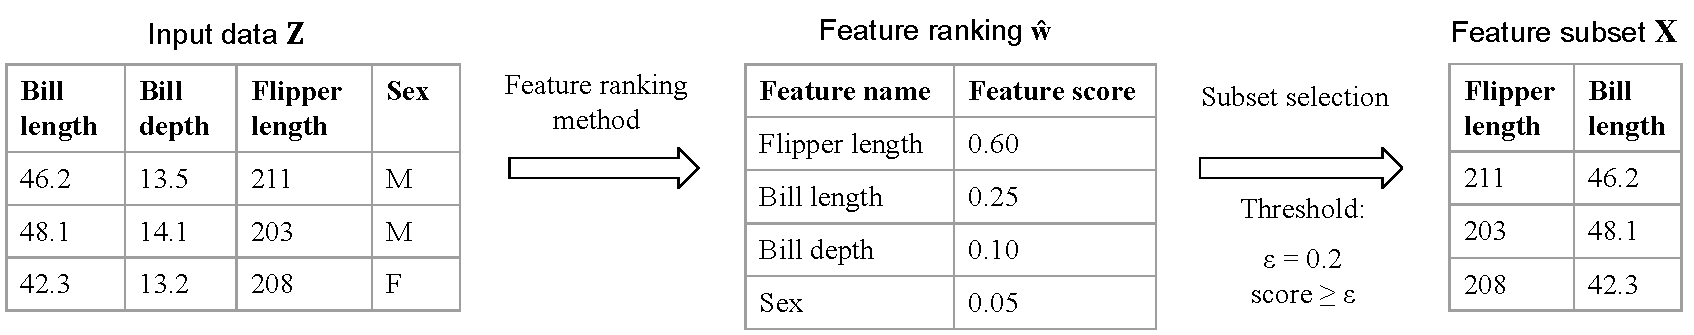
\includegraphics[width=\linewidth]{report/images/schematic-feature-selection.pdf}
    \caption{An example process of feature selection by thresholding a feature ranking at some point $\epsilon$. The resulting feature subset $\mathbf{X}$ presumably contains the strongest predictors given the target variable. Feature names come from a real dataset on antarctic penguins \citep{horst_palmerpenguins_2020}.}
    \label{fig:schematic-feature-selection}
\end{figure}

% so: feature ranking is important for feature selection -> they go hand in hand
For this reason, the more general problem of constructing feature rankings is omni-relevant in the feature selection domain - the only extra step necessary to finally arrive at the desired design matrix of reduced size is a sufficient threshold point, which many algorithms arrive at using different methods. A straightforward way to cut off low-ranking features is to exclude any feature that ranks below the mean score - or, alternatively, exclude only the highest ranking quartile, etcetera. More sophisticated schemes exist, however; one might also choose to iteratively run a feature ranking process and remove the lowest ranking score in each iteration (such a process is called \gls{rfe}). That said, it is clear that feature ranking and feature selection go in unison.

% (2) interpretable AI
\subsubsection{Interpretable Artificial Intelligence}
% algorithms became harder to reason about
The domain of Interpretable AI has been arisen due to the need to better understand and reason about the decisions that any Machine Learning model makes. Traditionally, the sole goal in building a learning algorithm would be to best predict some target variable, given some set of samples to learn from. With the advent of sophisticated learning algorithms such as Neural Networks and especially Deep Neural Networks, however, the many computational layers that separate inputs from answers tend to obfuscate the decision process \citep{rai_explainable_2020}. Whereas in classical statistical models practitioners sought to unveil a clear relationship between the independent- and dependent variables, some models in the field of Machine Learning have grown so complicated that no human can reason on its output. Because such algorithms tend to compare metaphorically to a black box one cannot possibly see through, one also refers to such algorithms as \textit{black boxes}.

% ML is used in professional world: we need transparency
Whilst at the same time models have gotten progressively more sophisticated and thus less transparent, the market for deploying Machine Learning has been steadily getting bigger. Many institutions seek to benefit from the possibilities of recent developments in \gls{ai} and \gls{ml} - including many companies, schools or the government. In all such applications, for every decision made by a Machine Learning model, an argumentation as how the model came to such a conclusion is desired. Even, in some scenarios the decision to be made at hand weighs so heavily that a \gls{ml} model that cannot explain itself might not be usable at all - think about a \gls{ml} model scoring employees such to fire the lowest ranking ones but providing only bare explanations on how it came to such a decision. As a matter of fact, faulty models of such kind have already been deployed out in the open - with considerable complications with respect to model transparency as a result \citep{oneil_weapons_2016}.

% interpretable AI to the rescue (two ways: (1) make model less complicated, (2) explain model)
For this reason, decisions made by computers are required to be explainable - allowing practitioners to assess not only \gls{ml} model decisions, but also assess the overall usefulness of the model in general. After all, many learning models are designed such to always generate a decision, no matter how noisy the input. That said, the black box of AI can generally be opened up in two ways. First, one could opt for a less sophisticated in the first place - one that reveals its inner workings and supports its decisions by an elaborate scheme, much in line with classical statistics. Although a simpler model could sometimes suffice in places where practitioners currently opt for more complicated ones, a solution for models of any kind of flexibility is desired. Therefore, a second option is to delve into any such model to reveal a reasoning about its decision-making process - which is the option that the field of Interpretable AI bothers itself with.

% feature rankings in interpretable AI
Feature rankings are one of the facets which can be used to facilitate a better understanding of a Machine Learning model \citep{hansen_interpretability_2019}: by unveiling which variables the \gls{ml} model finds important, a better understanding can be gained on its decision-making process. In some scenarios, it might, for example, be the case that the Machine Learning model in question unexpectedly weighs a feature as very important, even though a human expert can know apriori that the feature is not of value to the predictive task at hand. In this way, faulty models can be detected and prevented from being used in critical settings. In the Interpretable AI jargon, the process of scoring and explaining feature importance goes under different names. In the literature feature rankings are referred to as \textit{feature impact} scores, \textit{feature importance} scores, or \textit{feature effects} - they are synonymous in our case: all attempt to quantify feature relevance with respect to the learning task at hand. The general process of an interpretable AI algorithm can be seen as in Figure~\ref{fig:schematic-interpretable-ai}.

\begin{figure}[ht]
    \centering
    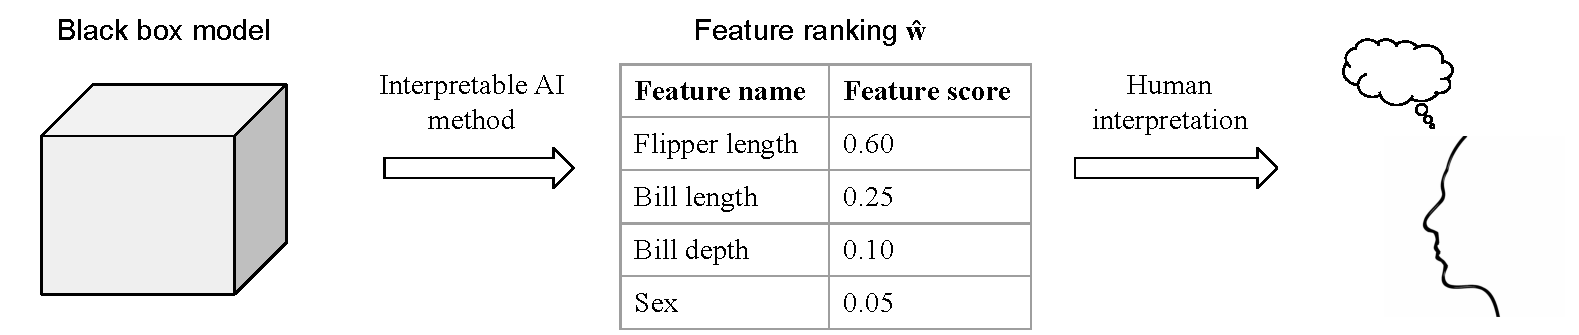
\includegraphics[width=\linewidth]{report/images/schematic-interpretable-ai.pdf}
    \caption{An example process of Interpretable AI. In this case, the input to the interpretable AI algorithm is a trained black box model, which decision making process is hard to understand otherwise. The interpretable AI algorithm then extracts feature importance scores for better interpretability.}
    \label{fig:schematic-interpretable-ai}
\end{figure}

% so: feature rankings are important for interpretable AI.
As could be seen in Figure~\ref{fig:schematic-interpretable-ai}, one way of making a black box model more interpretable is to extract a feature ranking from the trained model - an interpretable AI algorithm reads in the black box model and tries to explain it \citep{lundberg_unified_2017}. Other interpretable AI methods take a more direct approach \citep{arik_tabnet_2020}, in which the interpretable AI algorithm functions as a prediction method itself. The latter approach is employed only in more recent years; in which learning algorithms are designed from the start to be interpretable. However, independent of whether a direct- or indirect approach to explaining the decision process is taken, the desire to rank features is applicable to both. That said, we can therefore conclude that the construction of truthful feature rankings are an important aspect in interpretable AI.

\subsection{Motivations for Evaluating Feature Ranking methods}
Given the need for Feature Ranking methods, the desire to evaluate such methods systematically is clear-cut. Practitioners throughout the field of Machine Learning desire to know the behavior of different methods under a large range of varying conditions, such as dataset- sample size and dimensionality, dataset domains, the computational resources at hand and desired degree of accuracy of the solution. Finding out what evaluation- methods and metrics best represent the optimality of the solution is essential, for else the presentation of scientific findings might be misleading compared to real-world performance.

In this way, individuals and institutions are motivated to actively research Feature Ranking methods and evaluate them such to determine which method works best, under what conditions. As is more often the case in the comparison of Machine Learning algorithms, however, is the fact that methods are not always easily analytically compared - such that solely a theoretical analysis does not suffice to create a meaningful comparison. Although one can reason about the performance of many methods before conducting concrete data analyses, a real-world experiment is essential to any reputable publication.

\section{Related work}\label{section:related work}
% many papers in FS and Interpretable AI - but not so much on **evaluation**
The domain of feature- ranking and selection has a large availability of literature, spread out over many subtopics. What is more rare, however, is to find papers that explicitly research and reason about the usage of certain evaluation metrics. In general, papers tend to stick to a certain evaluation method when the majority employs the given technique - but a chance for conducting a more thorough analysis might be missed nonetheless.

% \subsection{Evaluation metrics in the Feature Selection domain}
%%% DOMAIN: feature selection
In the feature selection domain, the evaluation and comparison of feature selection algorithms is a non-trivial problem. Among a wide range of metrics, no consensus exists among researchers, leaving many papers to present outcomes in different ways \citep{guyon_introduction_2003}. In absence of a single consistent evaluation pipeline across the field, many scholars adhere to methods that are `widely used' \citep{solorio-fernandez_review_2020} \citep{li_feature_2017}.

Recommendations for metrics have been given in previous papers, most often when discussing future work. Arguments are made for relevant aspects to evaluate, such as in Chandrashekar (2014) \citep{chandrashekar_survey_2014}:

\begin{quote}\textit{"a feature selection algorithm can be selected based on the following considerations: simplicity, stability, number of reduced features, classification accuracy, storage and computational requirements"}\end{quote}

Of these aspects most proposals focus mainly on number of reduced features, classification accuracy and computational requirements. In the regression case, the classification accuracy would be replaced by a commonly used regression counterpart, the R2-score. Let us explore what validation estimators and corresponding metrics are used in papers across the field. Afterwards, evaluation aspects are covered that are not present in the aforementioned set.

\subsection{Evaluation metrics}
A \textbf{validation estimator} is often used to evaluate supervised feature selection methods; assessing the quality of a feature subset by running some predictor over the feature subset selected by the feature selection algorithm, obtaining the easily interpretable \textbf{prediction accuracy} metric in the classification case. Predictors often used in the literature include \gls{knn} \citep{al-tashi_review_2020} \citep{mafarja_dragonfly_2020}, \glspl{svm} \citep{chandrashekar_survey_2014}, \glspl{dt} \citep{li_feature_2017} and \gls{nb} \citep{koller_toward_1996}. Metrics used are often classification accuracy or in some cases average error rate \citep{khurma_evolopy-fs_2020}, validated using some $n$-fold cross validation, commonly 5- or 10-fold. See Table~\ref{table:evaluation-metrics-table}.

\renewcommand\theadalign{bl}
\begin{table}[ht]
    \centering
    \begin{tabular}{| l | l | l | l | l | l | l |}
    \hline
    \thead{Name method} & \thead{Validation \\ estimators} & \thead{Acc-\\uracy} & \thead{Stab-\\ility} & \thead{Time\\ $t(s)$} & \thead{Time\\ $\Omega(n)$} & \thead{Apriori\\info} \\
    \hline
    FOCUS \citep{almuallim_learning_1991}                       & \gls{dt}                              & Yes               & No                 & No                 & Yes                & No                    \\
    \hline
    Relief \citep{kira_feature_1992}                      & \gls{dt}                              & Yes               & No                 & Yes                & Yes                & No                    \\
    \hline
    Relief-F \citep{kononenko_estimating_1994}                    & \makecell[tl]{\acs{pcc}} & No                & No                 & No                 & No                 & Yes                   \\
    \hline
    INTERACT \citep{zhao_searching_2007}                    & \gls{dt}, \gls{svm}                         & Yes               & No                 & Yes                & Yes                & No                    \\
    \hline
    Fisher \citep{gu_generalized_2012}                      & \gls{knn}                            & Yes               & No                 & No                 & Yes                & No                    \\
    \hline
    MutInf \citep{zaffalon_robust_2014}                      & \gls{nb}                              & Yes               & Yes                & Yes                & Yes                & No                    \\
    \hline
    \makecell[tl]{Joint MutInf Maximization \citep{bennasar_feature_2015}}   & \gls{nb}, \gls{knn}                        & Yes               & Yes                & No                 & No                 & No                    \\
    \hline
    \makecell[tl]{Interaction Weight-based FS \citep{zeng_novel_2015}} & \makecell[tl]{\gls{dt}, \gls{ib1}, \gls{part}}                   & Yes               & No                 & Yes                & Yes                & Yes                   \\
    \hline
    \makecell[tl]{Infinite FS \citep{roffo_infinite_2015}}  & \gls{svm}                             & Yes               & Yes                & Yes                & Yes                & No                    \\
    \hline
    MultiSURF \citep{urbanowicz_relief-based_2018}                   &           -                      & No                & No                 & No                 & Yes                & Yes     \\
    \hline     
    \end{tabular}
    \caption{A comparison table of evaluation metrics used in Feature- Ranking or Selection paper proposals. Many different evaluation metrics are used, illustrating there exist no consensus on definite meaningful evaluation metrics in the field.}
    \label{table:evaluation-metrics-table}
\end{table}

\textbf{Stability}, on the other hand, is not widely used in theoretical or quantitative argumentation. Even though stability was recommended as a relevant evaluation metric by Chandrashekar (2014), not many papers explicitly argue for the stability of their method; the metric is called an \textit{"overlooked problem"} in Chandrashekar (2014). In many papers this metric is still regarded as a future work for solidifying any experimental results - the development of algorithms that achieve both high classification accuracy and high stability is still seen as a `challenging' problem by Tang et al (2015) \citep{tang_feature_2014}.

The trend seems to be turning though, with more authors becoming aware of the importance of stability. Our reliance on machine learning is ever-increasing, and so does the demand for interpretability and reliability of the algorithms. Take for example a biomedical application, in which feature selection is used to select genes in a gene sequencing analysis. Any expert in this domain field will feel more confident if an algorithm produces stable results given a varying sample population. This is how we define stability: given small changes in the sample data, the output of a feature selection process ought to be stable, i.e., the sensitivity of the selector to data perturbations. This metric for measuring an ability to generalize to achieving consistency has been long taken into account into prediction tasks, but not in feature selection - see for example Table~\ref{table:evaluation-metrics-table}.

\textbf{Scalability} is another point of attention that only recently caught more attention. The extra demand of algorithms to allow for parallel execution has been imminent as data grew tremendously large. Even, multi-core processing can lack in terms of performance, hence introducing the need for algorithms that can run in distributed fashion. Distributing a dataset over multiple machines poses challenges to some existing methods, though. Some current methods require the full dimensionality of the dataset to be available in-memory \citep{tang_feature_2014}. Yet, other methods require each sample to be visited multiple times, e.g., to apply a sample re-weighting strategy in order to converge. For these reasons, distributing any dataset workload on to multiple workers is a non-trivial problem; no generalized solution exists for cutting the dataset into chunks.

It is up to individual algorithms to find suitable ways of supporting parallel solutions and more importantly, support cases where data is too large to fit in-memory, i.e., apply distributed computing. Recent strategies overcome the issue of working with fewer samples by retaining only those samples that are most representative of the data - eliminating the need for working with a full sample population. Although few in number, there exist proposals for distributed dimensionality reduction methods \citep{li_distributed_2020}, using \textit{divide-and-conquer} techniques. Aggregating disjoint results would make for a performance similar to that of a centralized solution.

\subsection{Synthetic datasets and apriori information}
\textbf{Synthetic datasets} are employed in many papers in the literature. Whereas some datasets are injected by synthetically generated probe variables, others use completed generated benchmark datasets, such that benchmarks can be conducted in an even more controlled environment.
%... already pitched slightly by Guyon, e.g. "fake" variables.. + Solorio & Urbanowicz
About such partially synthetic datasets has been spoken of in literature since long, using datasets that are real but altered by injecting more data. In \citep{guyon_introduction_2003} the authors speak of \lq probe variables', which are used to discard any variable that scores lower than any of the probes. If the probe variables are set to be random variables, a simple way is obtained to apply a threshold to cut off features from the selected feature subset, i.e., by introducing known noise into the dataset we can construct more thoughtful cut-off thresholds.

Completely synthetic datasets, on the other hand, can allow for more sophisticated metrics to be used. Possibilities for new evaluation metrics are, for example described in \citep{solorio-fernandez_review_2020}: \textit{"Evaluation in terms of the redundancy of the selected features”} and \textit{“Evaluation in terms of the correctness of the selected features”}, the latter of which requires us to know what features are informative \textit{a priori} - which is accomplished with synthetic generation. Controlling all facets relevant to the quantitative analysis manually makes for a \textit{Simulation study}, which is argued for in \citep{urbanowicz_benchmarking_2018} as follows:

%... then move to Urbanowicz with examples from JMLR papers
\begin{quote}
    \textit{"Simulation studies such as these facilitate proper evaluation and comparison of methodologies because a simulation study can be designed by systematically varying key experimental conditions, and the ground truth of the dataset is known i.e. we know which features are relevant vs. irrelevant, we know the pattern of association between relevant features and endpoint, and we know how much signal is in the dataset."}
\end{quote}

Indeed, there seems to be a trend toward including synthetically generated datasets in experiments. In a review paper \citep{bolon-canedo_review_2013} the authors argue that synthetically generated datasets can yield statistically sound results because of the fact no inherent noise or redundancy will obstruct the experiment process. In other papers simulation studies are conducted as well \citep{cai_online_2020} \citep{tang_high-dimensional_2020} \citep{li_distributed_2020}, concluded by a small section depicting a `real data' analysis to conclude the point. For these reasons, a recommendation is made to include simulation studies in any comprehensive benchmark on feature ranking methods.

% \subsection{Evaluation metrics in the Interpretable AI domain}
%%% DOMAIN: interpretable AI

\section{Methods for Feature Ranking}\label{section:methods for feature ranking}
In the following, general theory related to the construction of feature rankings is discussed. The theory is required to be discussed because in order to best understand the evaluation process, an understanding of the construction process is a must.

\subsection{Terminology}
Among the subject of reducing dataset dimensions, there exists a common terminology that is used among the literature. Whilst some terminology is synonymous, other seemingly related terms mean different concepts entirely.

% feature selection versus feature ranking
\textbf{Feature Selection} and Feature Ranking are two terms often used interchangeably. Since often feature selection is done by first constructing a feature ranking and then cutting off features ranked lower than some threshold $\epsilon$, the construction of a feature ranking is often times an integral part of feature selection. Although feature selection methods exist that do not construct feature rankings, the two are synchronous in many ways, and are in this paper thus related to one another.

The term Feature Selection is used to indicate the general process of obtaining a feature subset with reduced size without transforming the data. Note that any feature selection method might transform the data in the algorithm however it likes internally - the stated terminology is only concerned with the eventual output of the feature selection algorithm. In this paper, a broad perspective is taken and not only feature selection methods but feature ranking methods generally are considered.

\textbf{Feature Ranking} is a broader term compared to Feature Selection, mapping onto more domains than just Feature Selection. Because in the construction of a Feature Ranking no assumptions are made on the desired data subset, a score is assigned to each of the dataset features, giving each dimension an `importance' score. Such scores can also be used to interpret and clarify a Machine Learning model: thus making such ranking processes useful to the interpretable AI domain.

% Categories of dimensionality reduction / feature screening / etc.
\textbf{Feature projection} and Feature Selection are both processes relating to the concept of dimensionality reduction \citep{cunningham_dimension_2007}, however, there exists an important distinction between them. Whilst in the process of feature selection, relevant dimensions are sought and selected without altering their input values, in the process of feature projection (also called \textit{feature extraction}) data transformations are applied, mapping the original data onto a lower-dimensional space. Common methods of feature projection are \textit{\gls{pca}} for the supervised case and \textit{\gls{lda}} for the unsupervised case. Both \gls{pca} and \gls{lda} take a statistical approach to detecting feature interactions, which not always results in an optimal feature set for prediction. Rather, machine learning techniques can be used to select a more optimal subset. Although the two methods are different, the two aim at achieving the same goal and are thus encountered in similar contexts.

\subsection{Types of Feature Rankings}\label{section:types of feature rankings}
To better understand in what form a Feature Ranking might be defined and how it relates to the process of Feature Selection, exact mathematical definitions of various types of feature rankings are given first. At all times, the prediction- or estimation of any quantity is denoted with a hat notation, i.e. `\textasciicircum', whilst the `true' value of the quantity has no such hat.

\subsubsection{Feature importance}\label{section:feature-importance-definition}
Feature importance scores are defined as a vector of $p$ dimensions, containing real-valued numbers. Let us define the vector like so:

\begin{equation}
\hat{\boldsymbol{w}} = (\hat{w}_1, \hat{w}_2, \ldots, \hat{w}_{p-1}, \hat{w}_p),
\end{equation}

where $\hat{\boldsymbol{w}} \in \mathbb{R}^p$. Such a ranking is obtained, for example, by running a feature ranker on the dataset and having it assigned as score to each dimension. The vector is assumed to be normalized, i.e. each vector element is divided by the vector sum:

\begin{equation}\label{eq:normalize-feature-ranking}
\hat{\boldsymbol{w}} = \frac{\hat{\boldsymbol{r}}}{\sum^p_{i=1} \hat{r}_i},
\end{equation}

given a scoring vector $\hat{\boldsymbol{r}}$, which indicates feature importance on an arbitrary scale. It is self-evident that $\hat{\boldsymbol{w}}$ has the property that $\sum^p_{i=1} \hat{w}_i = 1$, i.e. is a probability vector. An example such vector can be:

\begin{equation}\label{eq:importance-vector-example}
\hat{\boldsymbol{w}} = (0.20, 0.8, 0.0),
\end{equation}

in which it is clear that the ranking algorithm found the second feature to be the most important. In the case where multiple feature importance vectors are considered, e.g., in the case where $B$ bootstraps (Section~\ref{section:bootstrapping}) are considered, the vectors are stacked in a matrix, i.e.:

\begin{equation}\label{eq:feature-importance-matrix}
\mathbf{\hat{W}} \in \mathbb{R}^{B \times p},
\end{equation}

which denotes $B$ feature importance $p$-dimensional vectors arranged in a matrix of reals. The ground-truth $w$ will remain a vector, since there will still be only one such vector available per dataset.

\subsubsection{Feature support}\label{section:feature-support-definition}
Feature support indicates whether certain dimensions are chosen to be included a \textit{feature subset}; i.e. the vector marks elements as being chosen by the feature selection process. In this definition, the feature support vector is synonymous with the definition of a feature subset. Although some feature- ranking and selection processes approximate a suitable feature support vector directly, an algorithm can also make use of a threshold $\epsilon$ to generate a feature support vector from a feature importance vector. The feature support vector is a boolean-valued vector of $p$ dimensions.

\begin{equation}
\hat{\boldsymbol{s}} = (\hat{s}_1, \hat{s}_2, \ldots, \hat{s}_{p-1}, \hat{s}_p),
\end{equation}

where $\hat{\boldsymbol{s}} \in \mathbb{B}^p$. Note $\mathbb{B}$ is the boolean-valued vector space, i.e. its elements lie in the set $\{0, 1\}$. An example such vector can be:

\begin{equation}\label{eq:support-vector-example}
\hat{\boldsymbol{s}} = (1, 1, 0),
\end{equation}

which is the feature support mask obtained from thresholding the feature importance vector $\hat{\boldsymbol{w}}$ in the above example (Equation~\ref{eq:importance-vector-example}) using the threshold $\epsilon > 0.0$, causing one feature to be dropped from the feature subset. Just like for the feature importance vector, the feature support vectors can be arranged in a matrix in the boolean space, like so:

\begin{equation}\label{eq:feature-support-matrix}
\mathbf{\hat{S}} \in \mathbb{B}^{B \times p},
\end{equation}

given $B$ feature support vectors.

A \textbf{sparse representation} can also be constructed, given a feature support vector. A set is created containing only the indices of the selected features, causing a more sparse representation of the feature subset in case of high dimensionality and relatively few selected features. The support vector $\boldsymbol{s}$ and its prediction $\hat{\boldsymbol{s}}$ can be readily converted back- and forth into such a sparse representation. We define the sparse representation as the set $\hat{\mathbb{S}}$:

\begin{equation}
\hat{\mathbb{S}} = \{i \mid i \in \mathbb{Z} \wedge \hat{s}_i = 1 \},
\end{equation}

where $| \hat{\mathbb{S}} | = d$, i.e. $d$ dimensions were selected in the feature subset. Note, that the sparse feature subset is represented as a \textit{set} instead of a vector, meaning that the sequence is no longer considered ordered. To show a concrete example, the vector from Equation~\ref{eq:support-vector-example} is converted to the following set:

\begin{equation}
\hat{\mathbb{S}} = \{ 2, 1 \} \text{ where } | \hat{\mathbb{S}} | = 2,
\end{equation}

containing the indices of the selected features as defined in Eq~\ref{eq:support-vector-example}, in no particular ordering whatsoever. A sparse set $\hat{\mathbb{S}}$ can be converted back to a feature support vector $\hat{\boldsymbol{s}}$ like so:

\begin{equation}
\hat{s}_i = \begin{cases}
  1 & \text{if } i \in \hat{\mathbb{S}}\\
  0 & \text{otherwise}
\end{cases}
\end{equation}

Denote $B$ such sparse feature support sets as $\hat{\mathbb{S}}^{boot}$:

\begin{equation}\label{eq:feature-support-superset}
\hat{\mathbb{S}}^{boot} = \{ \hat{\mathbb{S}}_1, \hat{\mathbb{S}}_2, \ldots, \hat{\mathbb{S}}_{B-1}, \hat{\mathbb{S}}_B \},
\end{equation}

meaning $B$ sparse support sets were arranged in the superset $\hat{\mathbb{S}}^{boot}$.

\subsubsection{Feature rankings}\label{section:feature-rankings-definition}
Feature rankings are similar to feature importance scores, but with less precision. Whereas in a feature importance vector each element is approximated with a real-valued score, in an ordinary feature ranking the only considered facet is the \textbf{order} of the features in terms of importance. Although in most cases a feature importance vector is constructed first, after which a support or ranking vector can be constructed, in some cases only a ranking is available - e.g. in the case of \gls{rfe}. A feature ranking is constructed by assigning each dimension a rank, anywhere in the integer set $\{1, 2, \ldots, p - 1, p\}$. Such, the vector can be expressed as:

\begin{equation}
\hat{\boldsymbol{r}} = (r_1, r_2, \ldots, r_{p-1}, r_p),
\end{equation}

where $\hat{\boldsymbol{r}} \in \mathbb{Z}^p$, the integer-space. An example such vector can be:

\begin{equation}\hat{\boldsymbol{r}} = (2, 3, 1),\end{equation}

which is the feature ranking obtained from converting the feature importance vector $\hat{\boldsymbol{w}}$ in the above example (Eq~\ref{eq:importance-vector-example}) to a ranking. Such rankings are easily converted to importance vectors using Equation~\ref{eq:normalize-feature-ranking}, allowing one to use the same statistical machinery as for feature importance vectors. A higher rank number means a greater importance.

Such an integer-valued ranking can be utilised to select some $k$ best features to use in a subsequent learning task, i.e. to perform a feature subset selection. This is similar to selecting features using a threshold value $\epsilon$: now, however, a certain amount of features is selected - which is not the case for using a threshold value. Even though the feature- importance and ranking vectors both have the ability to select feature subsets, the feature importance vector carries more meaning, which can be made to good use during the evaluation process of the feature rankings using synthetically generated datasets, which will be elaborated upon later.

\subsection{Taxonomy}
Feature Rankings can be constructed by running a separate statistical operation on the dataset, before running any learning algorithms, or as part of a learning algorithm itself. In some cases, a learning algorithm that is itself very sophisticated and time-consuming might still be worthwhile to use as a feature selection pre-processing step - if time is saved by having the prediction estimator process less features, processing efficiency might be gained by using a feature selector.

Due to this distinction in the approach used in a feature ranking algorithm, a subdivision can be made to separate methods into more specific categories. As such, a common taxonomy in the field is created: subdividing feature ranking methods into the categories of filter-, wrapper- and embedded methods \citep{chandrashekar_survey_2014}.

\subsubsection{Filter methods}
Filter methods use some scoring mechanism to compute \lq usefulness' for each feature, without applying a learning algorithm. Having applied some ranking criterion, often a feature ranking is produced, after which some thresholding operation can be applied to select features. Although filter methods are often computationally light and do not overfit due to the absence of a learning algorithm, filter methods might miss out on more complex feature interactions, causing a non-optimal subset as a result. Also, choosing a suitable threshold to use can be difficult.

Examples of filter methods include the \textit{Fast Correlation Based Filter} \citep{yu_feature_2003}, which uses a quick and easy-to-compute statistical measure to select features according to some predefined threshold $\epsilon$ (in Yu et al. denoted as $\delta$). To illustrate the type of statistical quantities generally used in filter methods, the statistical quantity in Yu et al (2003) can be denoted like so:

\begin{equation}
S U(X, Y)=2\left[\frac{I G(X \mid Y)}{H(X)+H(Y)}\right],
\end{equation}

where $I G(X|Y)$ is the \textit{information gain} between two random variables $X$ and $Y$ and $H(X)$ is the \textit{entropy} of a variable: which are both metrics coming from the information-theoretical domain. The measure $SU(X, Y)$, then, is the \textit{symmetrical uncertainty} of two features $X$ and $Y$, where a feature $Y$ is more correlated to $X$ than to $Z$ if $IG(X, Y) > IG(Z, Y)$. In this way, a ranking can be constructed considering the measure $SU(X, Y)$, where feature are sought with high $SU$ scores. In a second phase of the algorithm, the scoring table is traversed yet again, to eliminate possible redundant features included in the selected feature subset.

\subsubsection{Wrapper methods}
Wrapper methods, on the other hand, use some learning algorithm to determine a suitable subset of features. A search is conducted over the space of possible feature subsets, eventually selecting the subset that has the highest validation score in the test set using a chosen learner as a predictor. Characteristics that define wrapper methods lend themselves similar characteristics to traditional optimisation problems; although an exhaustive search might yield an optimal solution, such a solution might not always be feasible due to its great time complexity. For this reason, in some applications a filter is applied first, before running a wrapper method.

Examples of such methods are numerous. Straight-forward methods include the range of \textit{sequential} feature selection methods, which aim to start (1) either with the full subset of dataset features or (2) with an empty set of features. The two approaches are called \textit{Forward} Feature Selection and \textit{Backward} Feature Elimination, respectively. To then facilitate a forward- or backward iteration step it is customary to use an estimator of some kind to retrieve a scoring on the features, selecting either the best- or eliminating the worst scored feature. \gls{rfe} is one such backward-elimination method, which might, for example, use a \gls{svm} to construct estimation scores \citep{maldonado_weber_2009}. Another option is to perform an exhaustive search, in which every feature combination is tried such to obtain the optimal feature subset, given the learning task and the estimator used. To obtain such a ranking, the chosen estimator might use an arbitrary method to compute it, be it a relatively simple learning step or a sophisticated model evaluation. Although such methods can perform reasonably well, such methods tend to be more time-consuming than filter methods.

\subsubsection{Embedded methods}
Embedded methods seek to combine the training task and feature selection. Given some suitable learner, features are weighted during the training process, producing either a feature ranking or a feature subset afterwards. e.g. some learners compute feature importance scores as part of their training process, which can then be used in combination with some threshold to select relevant features. Having already trained the model, subsequent prediction tasks can benefit from increased prediction speed by using less data.

Examples of embedded methods are \gls{lasso} and Ridge Regression, which perform feature selection alongside the process of finding optimal regression coefficients. For further explanations, see Section~\ref{section:ridge-regression}. Another notable embedded method is a \gls{dt}, which constructs, inherent during its fitting stage, a measure of importance on each variable. It does so by computing the probability of reaching a certain node - and determining the decrease in node impurity caused by weighting this probability value. To facilitate this computation, the probability of reaching a certain node is computed by considering the number of samples that reach the node during its decision-phase, divided by the total number of samples. Such, the leaves and depth obtained during the construction phase of the \gls{dt} can be used to determine a measure of feature importance, `embedded' into its learning phase.


\subsubsection{Hybrid methods}
A hybrid method is any method that is not classifiable by a single category, but rather lends from multiple categories. Hybrid methods can, for example, combine filter and wrapper methods \citep{hsu_hybrid_2011}, by first applying a computationally efficient filter and refining the result by using a wrapper method. Another paper \citep{das_filters_2001} describes its approach as hybrid due to both adding- and removing features in the feature selection process - exhibiting both forward- and backward selection at the same time. Lately, research was also put into examining \textit{Ensemble} feature selection methods \citep{bolon-canedo_ensembles_2019}, which combines the outputs of multiple selectors and decides useful features accordingly using some voting committee. Ensemble methods can be seen as hybrids or are seen as a category on its own.

\subsection{Types of features}
An important consideration in choosing a suitable feature selection method for any task is what kind of structure the concerning data has, if any at all. Data might exhibit tree, graph, or grouped structures, which is essential information when detecting feature interactions and determining useful features. Support for structured data is relatively new in the field and has not been an extensive point of concern for many feature selection algorithms in the past. Many traditional feature selection algorithms focused primarily `\textit{conventional flat}' features \citep{li_feature_2017}, in which the assumption is made that the data is independent and identically distributed (\textit{i.i.d.}). However, this assumption is widespread among many machine learning algorithms, since in many applications datasets are normalized to fit the i.i.d. condition before they are used.

Conventional data are opposed to more complex data structures, i.e., datasets with `structured features', as coined by the proposed taxonomy from J. Li et al (2017) \cite{li_feature_2017}, but also to linked data and \textit{streaming data}. In streaming data, the quality of an initially selected feature subset can be improved as more data comes in, and a feature selection algorithm is able to benefit from a larger distribution of samples. Adapting existing feature selection algorithms to fit the demands of streaming data proved to be a nontrivial problem. Nowadays, many companies and institutions have to deal with data volumes that easily exceed the boundaries of in-memory storage capacity - limiting the data scientist to train on only subsets of the entire datasets. Smart sampling is therefore needed to retain a representative sample distribution.

The scope of this research is limited to only the most common type of features, \textbf{conventional-, flat features} (\textit{i.i.d.}), or also \textit{tabular} data.

\subsection{Constructing Feature Rankings}
Although the number of existing feature ranking methods are numerous, a small set of example methods are explored to get a better understanding of the range of methods that do exist. First of all, a way of constructing a feature ranking that originates from classical statistics is examined. Next, a more algorithmic-type of approach is examined, which was specifically designed for the feature selection domain.

\subsubsection{Regularized Linear Regression}\label{section:ridge-regression}
One of the most fundamental methods in statistics is linear regression. It can be solved both analytically and numerically: in which the optimal approach is dependent on the amount of dataset dimensions at hand - where the amount of dataset dimensions $p$ gets very large, the analytic solution gets slower compared to an approximate method like Stochastic Gradient Descent. Recall that we can analytically solve Linear Regression by minimizing the Residual Sum-of-Squares cost function \citep{hastie_elements_2009}:

\begin{equation}\text{R}(\boldsymbol{\beta}) = (\mathbf{Y} - \mathbf{Z} \boldsymbol{\beta})^\intercal (\mathbf{Y} - \mathbf{Z} \boldsymbol{\beta}),\end{equation}

in which $\mathbf{Z}$ is our design matrix. Regression using this loss function is also referred to as `Ordinary Least Squares'. The mean of the cost function $\text{R}$ over all samples is called Mean Squared Error, or MSE. Our design matrix is built by appending each data row with a bias constant of 1 - an alternative would be to first center our data to get rid of the intercept entirely. To now minimize our cost function we differentiate $\text{R}$ with respect to $\boldsymbol{\beta}$, giving us the following unique minimum:

\begin{equation}\hat{\boldsymbol{\beta}} = (\mathbf{Z}^\intercal \mathbf{Z})^{-1} \mathbf{Z}^\intercal \mathbf{Y},\end{equation}

which results in the estimated least-squares coefficients given the training data, also called the normal equation. We can classify by simply multiplying our input data with the found coefficient matrix: $\hat{\mathbf{Y}} = \mathbf{Z} \hat{\boldsymbol{\beta}}$. Now, in the case where our model is fit using multiple explanatory variables, we are at risk of suffering from \textit{multicolinearity} - the situation where multiple explanatory variables are highly linearly related to each other causing non-optimal fitting of the model coefficients.

In \textbf{Ridge regression}, we aim to tamper the least squares tendency to get as `flexible' as possible to fit the data best it can. This might, however, cause parameters to get very large. We therefore like to add a penalty on the regression parameters $\boldsymbol{\beta}$; we penalise the loss function with a square of the parameter vector $\boldsymbol{\beta}$ scaled by new hyperparameter $\lambda$. This is called a \textit{shrinkage method}, or also: \textit{regularization}. This causes the squared loss function to become:

\begin{equation}\text{R}(\boldsymbol{\beta}) = (\mathbf{Y} - \mathbf{Z} \boldsymbol{\beta})^\intercal (\mathbf{Y} - \mathbf{Z} \boldsymbol{\beta})+\lambda \boldsymbol{\beta}^\intercal \boldsymbol{\beta},\end{equation}

where we can see that $\boldsymbol{\beta}^\intercal \boldsymbol{\beta}$ denotes the square of the parameter vector, thus supplementing the loss function with an extra penalty. This is called regularization with an $L^2$ norm; which generalization is called \textit{Tikhonov regularization}, which allows for the case where not every parameter scalar is regularized equally. If we were to now derive the solutions of $\boldsymbol{\beta}$ given this new cost function by differentiation w.r.t. $\boldsymbol{\beta}$:

\begin{equation}\hat{\boldsymbol{\beta}}^{\text {ridge }}=\left(\mathbf{Z}^{T} \mathbf{Z}+\lambda \mathbf{I}\right)^{-1} \mathbf{Z}^{T} \mathbf{Y},\end{equation}

in which $\lambda$ will be a scaling constant that controls the amount of regularization that is applied. Note $\mathbf{I}$ is the $p \times p$ identity matrix - in which $p$ are the amount of data dimensions used. An important intuition to be known about Ridge Regression, is that directions in the column space of $\mathbf{Z}$ with small variance will be shrunk the most; this behavior can be easily shown be deconstructing the least-squares fitted vector using a \gls{svd}. 

\textbf{\gls{lasso} regression} is a slightly modified variant of Ridge Regression, where instead of an $L^2$ norm an $L^1$ norm is used instead. This problem can be denoted as the following minimization problem:

\begin{equation}
\hat{\boldsymbol{\beta}}^{\text {lasso }}=\underset{\boldsymbol{\beta}}{\operatorname{argmin}}\left\{\frac{1}{2} \sum_{i=1}^{N}\left(y_{i}-\beta_{0}-\sum_{j=1}^{p} x_{i j} \beta_{j}\right)^{2}+\lambda \sum_{j=1}^{p}\left|\beta_{j}\right|\right\},
\end{equation}

in which the similarities between Ridge Regression are easily seen. The squared $\sum_1^p \beta^2_j$ ridge penalty is replaced by by the $L^1$ norm penalty of $\sum_1^p |\beta_j|$.

\textbf{Feature selection} can be employed using both \gls{lasso}- and Ridge regression. Because the dimensions whose coefficients are shrunk the most are presumably the least relevant to the prediction task, non-contributing features can be cut off from the design matrix using a threshold point. In fact, because \gls{lasso} does not square the weights vector but takes the absolute value, some coefficients might even be shrunk to near-zero values: removing the need for defining a threshold at all, since the coefficients have zero contribution already. In line with the feature subset definition given in Section~\ref{section:feature-support-definition}, such a feature support set can be constructed by thresholding the \gls{lasso} coefficients like so:

\begin{equation}
\hat{\mathbb{S}}^{lasso} = \{ j \mid \lvert \beta_j \rvert \geq \epsilon \},
\end{equation}

which will result in a feature support set containing only the indices of features where the coefficients were at least larger than $\epsilon$.

Although the former methods are suited for regression tasks only, regularization schemes are employed widely and have similar mechanics in these applications. Examples are numerous and include regularized Logistic Regression, regularized \glspl{svm} and regularized Neural Networks: employing regularization in any Machine Learning model is standard practice. In this way, we gained insight into a fundamental tool to estimate feature importance and shrinking the model coefficients using a regularization term - and more importantly, the fact that it can be employed for feature selection.

\subsubsection{Relief-Based Feature Selection algorithms}
The Relief-family of feature selection algorithms originates from a seminal paper by Kira et al. \citep{kira_feature_1992}, introducing the original version of the Relief algorithm. Over time, many variations on the Relief algorithm have been made, most notably ReliefF \citep{kononenko_estimating_1994}. In fact, so many variations on the algorithm were made that one can speak of \glspl{rba} in the literature \citep{urbanowicz_relief-based_2018}. Due to the overall architectural design of the algorithm, \glspl{rba} manage to rank features and optionally select a feature subset within a reasonable time-complexity domain and is often competitive when it comes to validation estimator performance.

The algorithm works by usage of an \textit{instance-based} learning method, considering one data sample at a time and updating statistics on feature importance. Given a training dataset $\mathbf{Z}$, $n$ samples, $p$ dimensions and a relevancy threshold $\epsilon$, Relief can compute a measure of feature importance in a finite amount of time. The essential concept is to compute the $p$-dimensional Euclidean distance for a randomly picked instance, iterating over all dataset samples and computing the \textit{nearest `miss'} and \textit{nearest `hit'} for every instance. Such a miss- or hit is defined to be either one of the positive- or negative dataset instances. To now compute how much `relevance' should be added for each feature given the closest hit- and miss, a subroutine is used, in which for every feature the \textsc{diff} between the randomly picked instance and nearest- hit and miss is computed and squared.

Once the iterations are complete, the summed weights for each feature are stored in a vector $\boldsymbol{w}^{relief}$. Once all $n$ samples have been traversed, the feature weights vector $\boldsymbol{w}^{relief}$ is normalized by dividing by the amount of samples $n$. In this way, a ranking is constructed - which can be converted into a feature subset by applying the threshold $\epsilon$ to the ranking. i.e., using the notation introduced in \ref{section:types of feature rankings}, a feature subset can be constructed like so:

\begin{equation}
\hat{\mathbb{S}}^{relief} = \{ i \mid \boldsymbol{w}^{relief}_i \geq \epsilon \},
\end{equation}

given some threshold $\epsilon$.
    
\section{Evaluating Feature Rankings}\label{section:evaluating feature rankings}
Like seen in Chapter~\ref{section:related work}, the evaluation of feature- ranking and selection methods is a nontrivial process, that has been conducted in many ways in the literature. Because of this reason, it is desired to acquire a general evaluation method that is applicable to all feature- ranking and selection methods - which is argued for to be a solid and scientifically sound evaluation process. In this chapter, a reasoning is given on which evaluation metrics are possibly sensible to use, after which a general recommendation on evaluation for different scenarios is given.

\subsection{Cross-Validation and Bootstrapping}\label{section:cv}
Several steps can be undertaken to provide more reliable estimates of the feature ranker performance. The goal is to prevent the practitioner to get promising but misleading results, whilst keeping the performance of the benchmarking process at a reasonable level.

\subsubsection{Cross-Validation}
% why CV
For almost any Machine Learning experiment, it is recommended to use some form of \gls{cv}. Because a model has the possibility to get `learn' the training data, evaluating the performance of an estimator on just the set of training data is dangerous practice. Evaluation metrics can be misleading, suggesting better model performance than is actually the case - when such a model is employed outside the realm of the training data, model generalization performance can turn out to be very poor. Thus, also in the context of benchmarking feature- ranking and selection algorithms, validation must be performed by holding out a set of the available data samples at hand.

% 5-fold and 10-fold cv
The most simple form of \gls{cv} is a training/testing split, in which the practitioner holds out one set of the example data for use in the testing phase - it is to be remain unseen by the model during the training phase. More robust methods include training the model multiple times on various training datasets and evaluating on the held out testing data. This can be done using 5-fold or 10-fold \gls{cv}, where, for example, in the case of 5-fold \gls{cv} \sfrac{4}{5}th of the data is reserved for training and \sfrac{1}{5}th for testing, repeated for each fold - so 5 times.

% beware: perform cv correctly
What is especially important in the process of conducting \gls{cv}, is that no operations are performed \textbf{before} having split the data, that can influence the experimental results. For example, in the scenario where one want to select variables to be included in some feature subset and run some prediction estimators afterward, a practitioner must be careful to split the data before the variable selection process. This is because otherwise, the predictive estimators might gain an unfair advantage due to having already seen the left out samples, i.e. they have already gained an advantage from the variable selection that was performed on the full dataset. This might cause skewed and misleading estimations of the error rate of the estimators - causing faulty models. Therefore, it is at all times important to keep in mind the `right' way of performing \gls{cv}: split first before running any operations that regard the dataset samples \citep{ambroise_selection_2002}.

\subsubsection{Bootstrapping}\label{section:bootstrapping}
% bootstrapping
Bootstrapping, on the other hand, is a similar but different process. Performing a bootstrap is a classical method for estimating statistical quantities regarding the learning process, such as variance, prediction error, or bias. The process works by resampling the dataset with replacement $B$ times, such to create $B$ different permutations of the dataset. Then, the learning process is repeated for each of the $B$ bootstrap datasets, i.e., refitting the estimators for each of the permuted datasets. If, for example, the designated dataset is denoted like $\mathbf{Z}=\left(z_{1}, z_{2}, \ldots, z_{b}\right)$ with each sample $z_{i}=\left(x_{i}, y_{i}\right)$, then the $b$-th bootstrap permutation of the dataset can be denoted as $\mathbf{Z}^{* b}$. Such, estimates can be made of, for example, the variance of some statistical quantity $S$ computed over the dataset $\mathbf{Z}$:

\begin{equation}\label{eq:variance-bootstrap}
\widehat{\operatorname{Var}}[S(\mathbf{Z})]=\frac{1}{B-1} \sum_{b=1}^{B}\left(S\left(\mathbf{Z}^{* b}\right)-\bar{S}^{*}\right)^{2},
\end{equation}

which can be seen to be the unbiased average of the statistical quantity $S$ over the $B$ bootstrap permutations of $\mathbf{Z}$. Note that the average value of the statistic $S$ is computed like so:

\begin{equation}\label{eq:average-bootstrap}
\bar{S}^{*}=\sum_{b} S\left(\mathbf{Z}^{* b}\right) / B,
\end{equation}

i.e. by averaging $S$ over the $B$ bootstraps. Like such, a reasonable estimate can be made of any statistical quantity computed over the dataset, as long as the quantity can be computed for any permutation on the dataset and enough computational resources are available to run $B$ repeated experiments on each of the permutations.

% bootstrapping for feature ranking
The practice of bootstrapping comes useful to the evaluation of feature- ranking and selection algorithms, allowing the practitioner to better estimate quantities that would previously be less reliable estimates. Examples of such quantities are the feature ranking algorithm stability, variance, or fitting time. Especially in assessing the algorithm stability, there exists an interest to know how the designated algorithm functions under conditions of varying samples. For this, bootstrapping is especially useful, since the exact data generating distribution at hand is often not available- meaning no more samples can be drawn from the distribution to generate a larger data population. In the lack of a data generating distribution, resampling with replacement offers a solution.

\subsection{Validation estimators}\label{section:validation estimators}
% validation estimators: how they work
A straight-forward way to evaluate the performance of a feature selection algorithm is to run the ranking algorithm, and subsequently run a `validation' estimator on the selected feature subset. The quality of the selected feature subset is then quantified through the performance of the validation estimator: when more informative and relevant features are selected, validation estimator performance presumably goes up. The validation estimator can be configured to be any classifier or regressor, dependent on the prediction task at hand, though often choices are made from a common set of estimators as can be seen in Table~\ref{table:evaluation-metrics-table}. 

% feature rankings
This idea can be extended to feature rankings. Many feature selection algorithms are in fact feature ranking algorithms and do not provide a built-in mechanism to perform feature subset selection - the algorithms allow a user to define the desired amount of features to be selected using a hyper-parameter, which then uses its feature ranking internally to construct a feature subset, like explained in Section~\ref{section:types of feature rankings}. It is therefore desired to also benchmark such algorithms in a systematic way: allowing more flexibility with respect to the evaluation process.

\begin{figure}[ht]
    \centering
    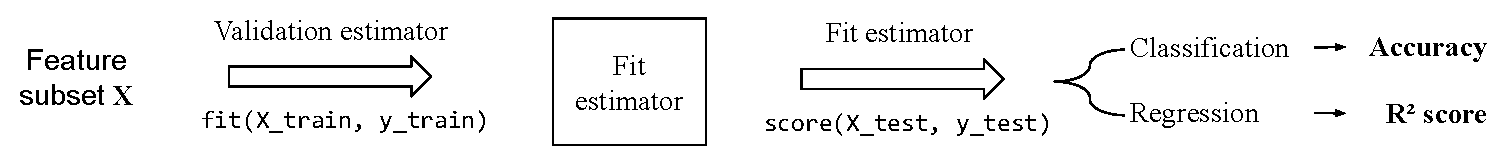
\includegraphics[width=\linewidth]{report/images/schematic-validation-estimators.pdf}
    \caption{The process of running a validation estimator on a feature subset. In the case of a feature ranking, a validation estimator is fit for some various amount of feature subsets. Often, feature subsets with some number of the highest ranked features are evaluated.}
    \label{fig:schematic-validation-estimators}
\end{figure}

As can be seen in Figure~\ref{fig:schematic-validation-estimators}, the process of running a validation estimator is straight-forward. Once a feature subset has been determined by thresholding a feature ranking or using the feature subset computed by a feature selection algorithm, a validation estimator is trained and evaluated on the held-out test set. Afterwards, a suitable evaluation metric is used depending on the learning task at hand: classification or regression (note the \hyperref[section:introduction]{research scope} was confined to just these two tasks). Exactly how many validation estimators are fit to evaluate a feature ranking depends on the ranking type (Section~\ref{section:types of feature rankings}). In the case of a feature support vector, only the feature subset might have to be evaluated, whilst for feature- importance or ranking vectors one might want to evaluate the first $k$ best feature subsets. Generally, each of the vectors are evaluated like so:

\begin{itemize}
    \item Feature importance vector (Section~\ref{section:feature-importance-definition}). Fit $k$ validation estimators, for the first $k$ best feature subsets, starting with a feature subset including only the highest ranked feature and subsequently including lower-ranked features. $k$ might be chosen depending on the dataset size at hand.
    \item Feature support vector (Section~\ref{section:feature-support-definition}). A feature subset was already selected by the feature selection algorithm and such the feature subset can be directly evaluated by the validation estimator.
    \item Feature ranking vector (Section~\ref{section:feature-rankings-definition}). A feature ranking can fit $k$ validation estimators; similarly to the feature importance vector.
\end{itemize}

Notably, in the case where a feature ranking algorithm supports computing both feature- importance or ranking vectors and the feature subset, i.e., the feature support vector, simply the $k$ best feature subsets can be evaluated by the validation estimator - assuming the selected feature subset to be included in one of the $k$ best feature subsets. If for some reason the selected feature subset $\hat{\mathbb{S}}$ is not in any of the $k$ best feature subsets, it will still be evaluated by a validation estimator separately.

A bootstrap can be used to generate more accurate estimations of the validation process. Especially for validation estimators that are sensible to varying permutations of the training data this process is useful - since otherwise validation metrics could be particularly misleading. In this way, given either an accuracy- or R\textsuperscript{2} score for classification and regression, respectively, an averaged bootstrapped score can be computed. This is done simply by plugging in either the R\textsuperscript{2} score or accuracy (or any other metric suitable for regression- or classification) into Equation~\ref{eq:average-bootstrap}.

\subsection{Apriori knowledge on relevant features}
% how to retrieve apriori info
In the scenario where we know \textit{\gls{apriori}} which features are relevant, more direct evaluation can be applied on the constructed feature ranking. Such apriori ground-truth information can be gained in a couple of ways: (1) by utilising human domain expert knowledge, (2) by augmenting real-world datasets with noisy dimensions and assuming all other dimension to be uniformly relevant or lastly (3) by generating synthetic datasets with known feature importance levels (see Section~\ref{section:pipeline-components-datasets}. In the context of this section, the assumption is made that the feature importance scores are simply `known' apriori: no restriction is made on exactly how feature relevance ground truth was retrieved.

% why its better
Knowing the relevant dataset features apriori can be useful information to the feature ranking evaluation process. This is because even though the goal of feature- ranking and selection algorithms is to separate the useful from the irrelevant features, the performance of such a ranking is nowadays most commonly evaluated by training yet another estimator; the `validation' estimator (Section~\ref{section:related work} and Section~\ref{section:validation estimators}). This makes the evaluation scores dependent on the validation estimator, requiring publications to have run the same validation estimator to make the results comparable between papers. Also, for some datasets, the chosen validation estimator might be sophisticated enough to make up for any noisy dimensions that were added - reducing the differences between the feature rankings, which is instead desired to be amplified to determine which feature ranker is the best for which dataset. Lastly, a sophisticated validation estimator might also perform a form of feature selection on its own, which might also skew the performance of faulty feature rankings that included lots of noisy dimensions in its feature subset. For these reasons, it is interesting to investigate the possibilities to find robust and reliable evaluation methods that do not require a validation estimator.

% evaluation using the ground-truth
Using the ground-truth relevant features, an accompanying evaluation metric can be constructed. Taking into consideration how different feature ranking algorithms construct various types of feature rankings as described in Section~\ref{section:types of feature rankings}, a suitable metric can be created for each.

% feature importance
\textbf{Feature importance} (Section~\ref{section:feature-importance-definition}) scores are defined to be a real-valued $p$ dimensional vector, $\hat{\boldsymbol{w}}$. In order to evaluate the closeness of the vector $\hat{\boldsymbol{w}}$ to the dataset ground truth $\boldsymbol{w}$, a range of metrics can be used. A first approach would be to regard the estimated vector as an estimation of a continuous target vector, i.e., to regard the problem as a regression type of task. In such a perspective, each predicted feature importance would pose as a data sample. In this way, usual metrics related to the regression task can be used.

The \textbf{R\textsuperscript{2}-score} is one such metric that can be used in this context. This can be formalized like so:

\begin{equation}
\begin{aligned}
R^{2}&=1-\frac{\mathrm{RSS}}{\mathrm{TSS}} \\
\text{where}&\\
\mathrm{RSS} &= \sum_{i=1}^{n}\left(y_{i}-f\left(x_{i}\right)\right)^{2} =\sum_{i=1}^{p}\left(w_i - \hat{w_i} \right)^{2}, \text{ and}\\
\mathrm{TSS} &= \sum_{i=1}^{n}\left(y_{i}-\bar{y}\right)^{2} =\sum_{i=1}^{p}\left( w_i - \bar{\boldsymbol{w}} \right)^{2}, \\
\end{aligned}
\end{equation}

which can be used to evaluate the closeness of the predicted feature importance vector $\hat{\boldsymbol{w}}$ to the ground-truth feature importance vector $\boldsymbol{w}$.

The \textbf{logistic-loss}, or \textit{cross-entropy} score is another metric which can be employed to quantify the quality of a feature importance vector $\hat{\boldsymbol{w}}$. In this scenario, however, the target variables are regarded to be binary labels, which therefore means the predicted feature importance vector $\hat{\boldsymbol{w}}$ is to be compared against $\boldsymbol{s}$ instead of $\boldsymbol{w}$. Remember, from Section~\ref{section:feature-support-definition}, that $\boldsymbol{s}$ is the $p$-dimensional vector indicating with a boolean whether or not the feature is relevant, i.e. $\boldsymbol{s} \in \mathbb{B}^p$. Such, a zero indicates a feature is not relevant; and a one indicates the feature is informative or relevant. In this way, a feature ranker approximates the true binary relevance labels $\boldsymbol{s}$ with probability values arranged in the probability vector $\hat{\boldsymbol{w}}$. The logistic loss can be formalized like so:

\begin{equation}
\begin{aligned}
L_{\log }(y, p) &= -\log \operatorname{Pr}(y \mid p)=-(y \log (p)+(1-y) \log (1-p)) \\
&\text{substituting for } s_i \text{ and } \hat{w_i}\\
L_{\log }(s_i, \hat{w_i}) &= -\log \operatorname{Pr}(s_i \mid \hat{w_i})= -(\hat{w_i} \log (\hat{w_i})+(1-s_i) \log (1-\hat{w_i})) \\
&\text{averaged over all vector components }\\
L_{\log }(\boldsymbol{s}, \hat{\boldsymbol{w}}) &= - \frac{1}{p} \sum_{i=1}^p (\hat{w_i} \log (\hat{w_i})+(1-s_i) \log (1-\hat{w_i})) \\
\end{aligned}
\end{equation}

% feature support
\textbf{Feature support} (Section~\ref{section:feature-support-definition}) is evaluated differently. Just like in the logistic-loss metric, the ground truth relevant labels are encoded as binary labels, i.e. the vector $\boldsymbol{s}$ is used as the ground-truth. Now, however, the predicted targets are also encoded as binary labels, i.e. the vector $\hat{\boldsymbol{s}}$ is used. This means that the problem is to be viewed in the supervised classification perspective and all metrics accompanying such task are available.

Classification \textbf{accuracy} is such a metric, measuring simply the average number of correct predictions were made between the predicted- and true target labels. It can be defined as such:

\begin{equation}
\begin{aligned}
\operatorname{accuracy}(y, \hat{y}) &= \frac{1}{n} \sum_{i=1}^{n} \boldsymbol{1} \left(\hat{y}_{i}=y_{i}\right) \\
&\text{substituting for } s_i \text{ and } \hat{s_i}\\
\operatorname{accuracy}(s, \hat{s}) &= \frac{1}{p} \sum_{i=1}^{p} \boldsymbol{1} \left(\hat{s}_{i}=s_{i}\right), \\
\end{aligned}
\end{equation}

where $\boldsymbol{1}(x)$ is the indicator function \citep{davis_undecidable_2004}. Using this metric, the amount of useful features included in a feature subset is rewarded with higher accuracy scores accordingly.

% feature ranking
\textbf{Feature rankings} (Section~\ref{section:feature-rankings-definition}) can be evaluated similarly to feature importance scores - thereby also requiring normalization. Presume that besides the relevance of the features is known as a binary value, also the \textit{order} of relevance is known, i.e. which features are more relevant than others. This is very similar to the feature importance scores: though the difference is that the feature importance scores must first be converted to a ranking such to allow for meaningful comparison. In this reasoning, both the predicted- and the ground truth feature ranking vectors, which are $\hat{\boldsymbol{r}}$ and $\boldsymbol{r}$ respectively, can be normalized using Equation~\ref{eq:normalize-feature-ranking} to obtain $\hat{\boldsymbol{w}}$ and $\boldsymbol{w}$, respectively.

% normalized
In this way, the normalized vectors $\hat{\boldsymbol{w}}$ and $\boldsymbol{w}$ can again be considered probability vectors, such that metrics like the R\textsuperscript{2}-score can be used: just like for the feature importance scores.

% mind: do not compare to importance scores
One has to keep in mind, however, not to intermix the feature importance and feature ranking scores with each other: even though the same metric is used to convert to summarize the predicted feature- importance and ranking vectors into a single scalar, the scorings are built from different vectors to begin with. The R\textsuperscript{2}-score coming from the feature importance vectors might have an unfair advantage due to the fact that they have floating-point precision on their approximations, whilst the feature ranking vectors $\boldsymbol{r}$ are converted from the integer domain to be normalized into floating-point numbers.

\subsection{Stability}
The stability of any algorithm is an important facet of the total method performance - which must not be overlooked or forgotten. This is for in many applications, only robust algorithms can be systematically relied on. Although it is only natural for algorithms to vary in fitting behavior under different permutations of the sample set, it is at all times desired to get an algorithm that is as stable as possible. To evaluate the stability of feature ranking algorithms, an easy method is to take several bootstrap permutations of the dataset (Section~\ref{section:bootstrapping}), to simulate drawing new samples from the data generating distribution at hand. Assuming such a bootstrapping procedure to be in place, several metrics can be used to quantify stability.

\subsubsection{Stability of feature importance vectors}\label{section:feature-importance-stability}
Feature importance scores are defined to be $p$ dimensional vectors in the domain of real numbers $\mathbb{R}$ (Section~\ref{section:feature-importance-definition}). Accordingly, the matrix containing $B$ such vectors is the $B \times p$ dimensional matrix in $\mathbb{R}$, denoted as $\hat{\mathbf{W}}$. A straight-forward way to assess the stability of the feature importance matrix is to compute the variance for each of the $p$ dimensions over $B$ bootstraps, i.e. Eq~\ref{eq:variance-bootstrap} is used by plugging in a column of the feature importance matrix $\hat{\mathbb{W}}$ as the statistical quantity $S$:

\begin{equation}
\widehat{\operatorname{Var}}[\hat{\mathbf{W}}_{:,i}]=\frac{1}{B-1} \sum_{b=1}^{B}\left(\hat{W}_{b,i}-\bar{\hat{\mathbf{W}}}_{:,i}^{*}\right)^{2},
\end{equation}

where $\bar{\hat{\mathbf{W}}}_{:,i}^{*}$ is the average feature importance score for the $i$-th feature over $B$ bootstraps. In this way, the variance over each dimension can be computed for a single feature ranker.

To summarize the variances over all dimensions, their summation might be taken, i.e., the variances are summarized as the scalar $\sum_{i=1}^p \widehat{\operatorname{Var}}[\hat{\mathbf{W}}_{:,i}]$. Alternatively, one might want to weight such summation, in order to reflect the desire to penalize instabilities in the ranking of relevant features more so than instabilities in the ranking of irrelevant features. In the case where the ground-truth feature importance scores are given, i.e. $\boldsymbol{w}$ is known, this vector might be used to apply a weighting scheme to the summation of the variances. One can do so by taking the inverse normalized ground truth feature importance score, i.e. $\frac{1}{w_i}$ for the $i$-th feature. Such, the summarization of $\hat{\mathbf{W}}$ now becomes $\sum_{i=1}^p \frac{1}{w_i} \widehat{\operatorname{Var}}[\hat{\mathbf{W}}_{:,i}]$.

\subsubsection{Stability of feature support vectors}
This time around, a way to quantify the stability of a feature subset is desired, i.e., the feature support vector $\hat{\boldsymbol{s}}$. A measure for the quantifying stability of set permutations that comes easily to mind might be the Hamming distance between multiple pairs of algorithm runs, i.e. ran on the same dataset with varied sample populations. Indeed, in \citep{dunne_solutions_2002} a measure based on Hamming distance is proposed. Reports also exist on numerous other approaches, like an entropy based measure \citep{krizek_improving_2007}, a measure based on the cardinality of intersection measure \citep{kuncheva_stability_2007} and a measure based on correlation coefficients \citep{kalousis_stability_2007}.

\textbf{Desired properties} of any measure are important to define in concrete manner. To compare the strength of any of these measures, the general objective for exactly what information we want to convey in a stability metric should be verbalized first. In \citep{mohana_chelvan_survey_2016}, three desired stability metric properties are expressed: (1) \textit{Monotonicity}, (2) \textit{Limits} and (3) \textit{Correction for chance}. Given the proposed measures in the literature, only few measures satisfied all properties. In another paper \citep{nogueira_stability_2017}, however, the authors extend the set of desired properties to include another two: (4) the stability estimator must be \textit{Fully defined} and (5) \textit{Maximum Stability $\leftrightarrow$ Deterministic Selection} - meaning that a maximum stability value should be achieved if-and-only if all feature sets are exactly identical.

\textbf{A measure} for quantifying feature subset stability was proposed in \citep{nogueira_stability_2017}, using the set of newly proposed desired properties. Having explored a statistically sound method to define a metric satisfying all five properties, the authors proposed a novel stability estimator, adjusted to this paper's terminology:

\begin{equation}\label{eq:stability-measure}
\hat{\Phi}(\hat{\mathbb{S}}^{boot})=1-\frac{\frac{1}{p} \sum_{i=1}^{p} \sigma_{i}^{2}}{\mathbb{E}\left[\frac{1}{p} \sum_{i=1}^{p} \sigma_{i}^{2} | H_{0}\right]}=1-\frac{\frac{1}{p} \sum_{i=1}^{p} \sigma_{i}^{2}}{\frac{\bar{k}}{p}\left(1-\frac{\bar{k}}{p}\right)},
\end{equation}

where $\hat{\Phi}$ resembles the stability estimate of the feature subsets arranged in $\hat{\mathbb{S}}^{boot}$ (Eq~\ref{eq:feature-support-superset}). Remember, that each set in $\hat{\mathbb{S}}^{boot}$ is a feature subset containing the indices of the selected features. Each of the sets in $\hat{\mathbb{S}}^{boot}$ is created by running the feature ranker on a permutation of the datasets, i.e. a resampling of a dataset equal probability distribution and dataset properties. Furthermore, the authors define $\sigma_{i}^{2}$ as the unbiased sample variance of the selection of the $i^{t h}$ feature and $\bar{k}$ as the average number of features selected over the $B$ feature sets. Given this paper's goal, there is no necessity for going into further mathematical details - for this we refer to the paper itself.

What is important is that this new measure satisfies all desirable properties for quantifying stability, as was proven in the paper. Accompanying the novel definition are instructions for computing confidence intervals and for performing a hypothesis testing for comparing various method stabilities. Exploring feature selection stability values given a set of parameter choices not only allows for choosing better hyperparameters, but also allows for comparing stabilities over various feature selection methods.

\subsubsection{Stability of feature ranking vectors}
Lastly, the stability of feature ranking vectors is also to be quantified. Since the stability measure for feature support was all about working with sets instead of vectors, the best option is to again normalize to a feature importance vector and compute the variance thereof. The summarization of the variances might again be weighted using the ground-truth feature importance vector $\boldsymbol{w}$, if it is available. See Section~\ref{section:feature-importance-stability}.

\subsection{Time complexity}
Another metric to be taken into account is algorithm complexity, which manifests itself in three interlinked aspects: time-, storage- and algorithm simplicity. Like the classical principle \textit{Occam's razor} implies - there at all times exists a preference for simpler models over more complex ones, especially in the case both accomplish the same feat. So, an understandable model is preferred that performs limited computational steps in order to restrain time- and storage complexity from rising too high.

Although measuring algorithm time- and storage requirements does provide some understanding, more insightful would be a theoretical description of the complexity in Big O notation. Theoretical complexities are harder to obtain though - leaving many authors to resort solely to measurements. Nonetheless, complexity analysis is recommended to be part of any feature selection method comparison, for it is a critical aspect to consider.

\subsection{Statistical integrity}
Given that the above discussed evaluation methods are computed, a statistical test is ought to be applied to provide convincing evidence for any algorithm's superiority. Like explained in \citep{demsar_statistical_2006}, many papers make implicit hypotheses acclaiming improved performance over existing methods. Although the chosen metrics might have been appropriate to statistically show performance gains as significant, the results are less reliable when left not validated by a statistical test. Therefore, a statistical verification step is required in the feature selection evaluation process.

Comparing multiple feature selectors is a non-trivial problem, which can be seen as the problem of comparing multiple \textit{classifiers}. To compare multiple classifiers, \citep{demsar_statistical_2006} recommends the Wilcoxon signed ranks test for comparison of two classifiers and the Friedman test for comparison of more classifiers given multiple datasets. Accompanying the Friedman test, it is recommended to perform corresponding post-hoc tests, such as the Nemenyi test \citep{nemenyi_distribution-free_1963}. The usually popular ANOVA test was advised against because, given the context of machine learning, ANOVA assumptions are violated, e.g. ANOVA assumes samples are drawn from normal distributions and the requirement of random variables having equal variance.

A \textbf{Wilcoxon signed ranks test} and the \textbf{Friedman test}, are for these reasons recommended for two- or more methods respectively, to statistically verify significant differences in performance of feature selection algorithms over the others using some summarizing scalar per feature selection method per dataset. The Friedman test is recommended to be accompanied with a post-hoc test, like Nemeyi's post-hoc test.

% PIPELINE
\section{Building a benchmarking pipeline}\label{section:pipeline}
To facilitate conducting a comprehensive experiment, many experiments must be run. To do so, a pipeline is to be built - supporting computing the required metrics, visualizing the results, and doing so whilst being scalable. 

\subsection{Architecture}
% schematic of all components; how the pipeline works
% ... data flow schematic


\begin{figure}[h]
    \centering
    % https://docs.google.com/drawings/d/11qgqcMbxe6vyU8cv9KAZLeJPodVBi64TQCDwtNJp09g/edit
    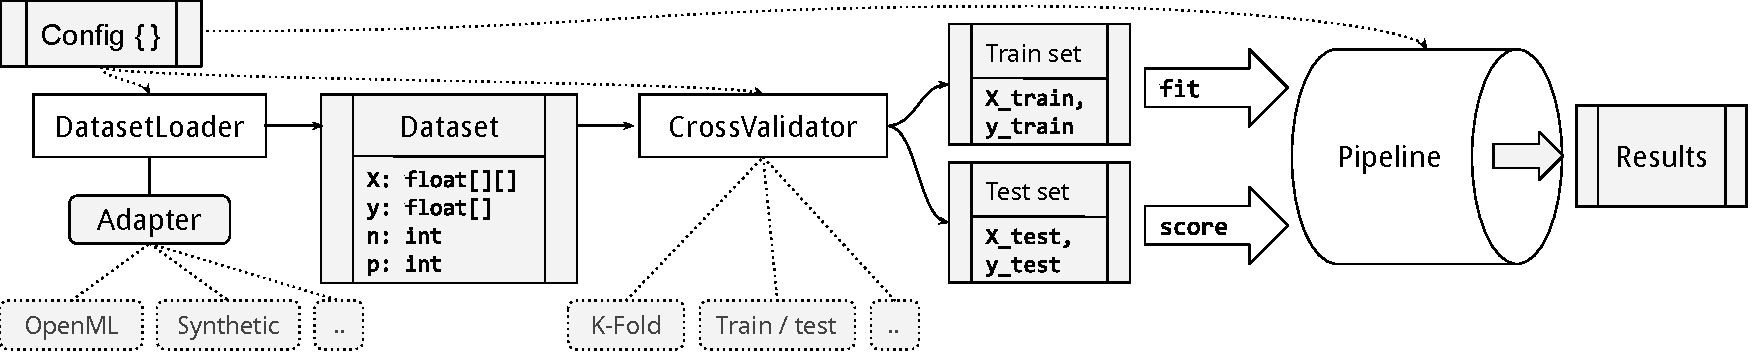
\includegraphics[width=\linewidth]{report/images/schematic-main-architecture.pdf}
    \caption{A general architecture schematic of the built benchmarking pipeline. Once the designated dataset is loaded using a configured adapter, the data is fed to the pipeline after a \gls{cv} split. The pipeline is first fit using the training data and then scored using the testing data.}
    \label{fig:schematic-main-architecture}
\end{figure}

\begin{figure}[h]
    \centering
    % https://docs.google.com/drawings/d/103YO-SX4JcwK_DbdT6G365ffvHJ7xCJQGaoUMoSvpeg/edit
    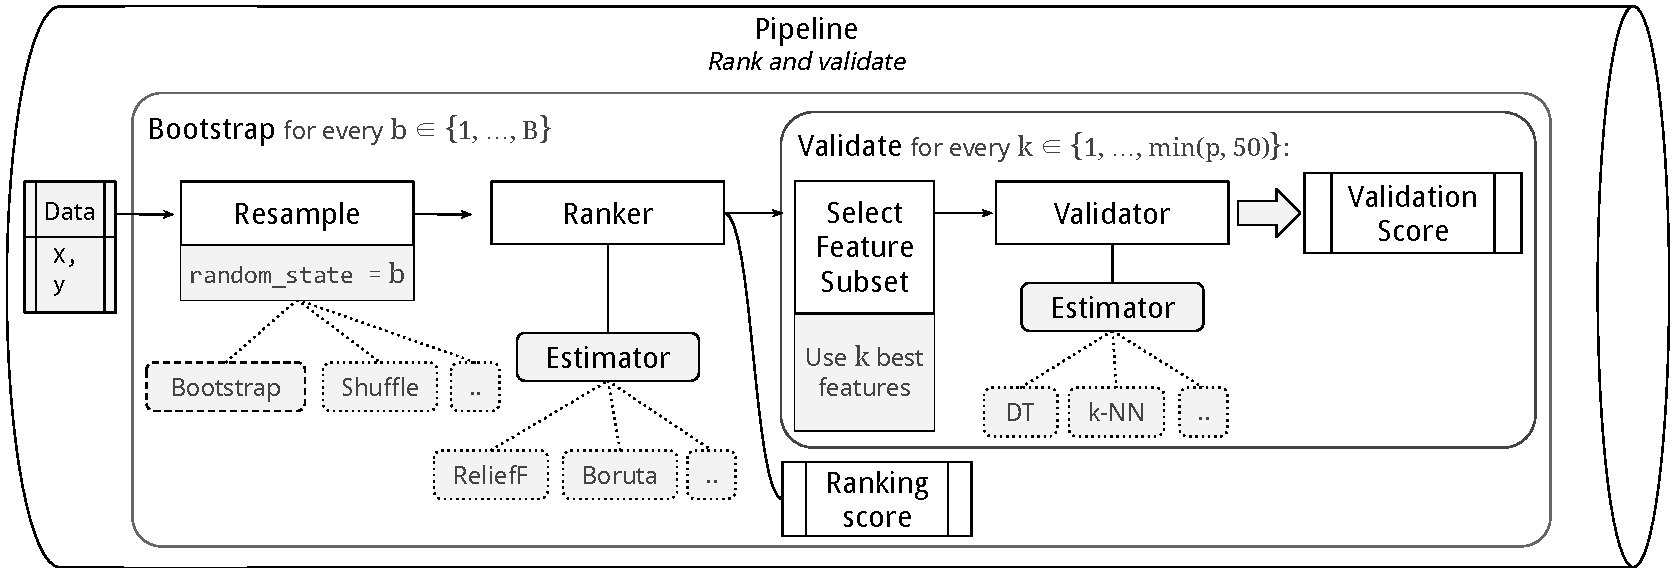
\includegraphics[width=\linewidth]{report/images/schematic-pipeline-architecture.pdf}
    \caption{.}
    \label{fig:schematic-pipeline-architecture}
\end{figure}

\subsection{Components}
\subsubsection{Datasets}\label{section:pipeline-components-datasets}
% adapters & storing datasets

\subsubsection{Cross-Validation}
\subsubsection{Resampling}
\subsubsection{Estimators}
\subsubsection{Storage providers}
\subsubsection{Callbacks}

\subsection{Configuration}
% hydra, etc

\subsection{Execution}
\subsubsection{Multiprocessing}
\subsubsection{Distributed computing}
\subsubsection{Caching}

\subsection{Monitoring}
% wandb/etc



% EXPERIMENTS
\section{Experiments}\label{section:experiments}
\subsection{Experiment setup}
% In the case of evaluating a feature ranking, a validation estimator is run for at most $\min\{50, p\}$ feature subsets. Such feature subsets include the highest $\min\{50, p\}$ ranked features: with each feature subset including the next lesser-ranked feature, starting with a feature subset that only includes the number one highest ranked feature.
\subsubsection{Experiment design}
\subsubsection{Feature Rankers lineup}
\subsubsection{Datasets lineup}

\subsection{Individual experimental results}
\subsection{Aggregated experimental results}

\section{Discussion}\label{section:discussion}
\section{Conclusion}\label{section:conclusion}
\subsection{Concluding note}
\subsection{Future work}

\bibliographystyle{abbrv}
\bibliography{references}

\begin{appendices}

\end{appendices}
\clearpage

\glsaddall
\printnoidxglossary

\end{document}
